%-----------------------------------------------------------------------
%
% File Name: thesis.tex
%
% Author: Lough, J. D.
%
%
%-----------------------------------------------------------------------

% document class and packages
\documentclass[12pt,notitlepage]{report}
\usepackage{bibunits}
\usepackage{syrthesis}
\usepackage{graphicx}
\usepackage{subfigure}
\usepackage{array}
\usepackage{multirow}
\usepackage{color}
\usepackage{amsmath}
\usepackage{amssymb}
\usepackage{amsfonts}
\usepackage{tensor}
\usepackage{acronym}
\usepackage{listings}
\lstset{breaklines=true,
  basicstyle=\ttfamily\footnotesize}
\usepackage{lscape}
\usepackage{hyperref}
\usepackage{dsfont}
\usepackage[disable,colorinlistoftodos]{todonotes}
\usepackage{tikz}
\usepackage{pgfplots}
\pgfplotsset{width=14cm,compat=1.6}
\usetikzlibrary{external}
%\tikzexternalize[prefix=tikz/,mode=list and make]
\tikzexternalize[prefix=tikz/]


% journal definitions
\newcommand{\apj}{{\it Astrophysical J.}}
\newcommand{\apjl}{{\it Astrophysical J.}}
\newcommand{\aap}{{\it Astron. and Astrophys.}}
\newcommand{\cmp}{{\it Commun. Math. Phys.}}
\newcommand{\grg}{{\it Gen. Rel. Grav.}}
\newcommand{\cqg}{{\it Class. Quant. Grav.}}
\newcommand{\lr}{{\it Living Reviews in Relativity}}
\newcommand{\mnras}{{\it Mon. Not. Roy. Astr. Soc.}}
\newcommand{\pr}{{\it Phys. Rev.}}
\newcommand{\prl}{{\it Phys. Rev. Lett.}}
\newcommand{\pra}{{\it Phys. Rev. A}}
\newcommand{\prd}{{\it Phys. Rev. D}}
\newcommand{\nat}{{\it Nature}}
\newcommand{\prsl}{{\it Proc. R. Soc. Lond. A}}
\newcommand{\ptrsl}{{\it Phil. Trans. Roy. Soc. London}}
\newcommand{\rmp}{{\it Rev. Mod. Phys.}}

% acronymn definitions
\acrodef{LIGO}{Laser Interferometer Gravitational-wave Observatory}
\acrodef{BNS}{binary neutron star}
\acrodef{BBH}{binary black hole}
\acrodef{NSBH}{neutron-star black-hole binary}
\acrodef{FAR}{\emph{false alarm rate}}
\acrodef{IFAR}{inverse false alarm rate}
\acrodef{SNR}{signal-to-noise ratio}
\acrodef{MM}{minimal match}
\acrodef{IFO}{interferometer}
\acrodef{CBC}{compact binary coalesence}
\acrodef{GW}{gravitational wave}
\acrodef{PDF}{probability distribution function}
\acrodef{S5}{LIGO's fifth science run}
\acrodef{S6}{LIGO's sixth science run}
\acrodef{VSR1}{Virgo's first science run}
\acrodef{VSR2}{Virgo's second science run}
\acrodef{VSR3}{Virgo's third science run}
\acrodef{pN}{post-Newtonian}
\acrodef{LVC}{LIGO Scienctific Collaboration and the Virgo Collaboration}
\acrodef{DAG}{directed acyclic graph}
\acrodef{HIPE}{Hierarchical Inspiral Pipeline Executable}
\acrodef{HIPE}{Hierarchical Inspiral Pipeline Executable}
\acrodef{SPA}{stationary-phase approximation}
\acrodef{ISCO}{the inner-most stable circular orbit}
\acrodef{FFT}{Fast-Fourier Transform}
\acrodef{LLO}{LIGO Livingston Observatory}
\acrodef{LHO}{LIGO Hanford Observatory}
\acrodef{LSC}{LIGO Scientific Collaboration}
\acrodef{DQ}{data quality}
\acrodef{LLF}{local Lorentz frame}
\acrodef{GR}{General Relativity}
\acrodef{EM}{electromagnetic}
\acrodef{pdh}[PDH]{Pound Drever Hall}
\acrodef{psl}[PSL]{Pre-Stabilized Laser}
\acrodef{iss}[ISS]{Intensity Stabilization Servo}
\acrodef{fss}[FSS]{Frequency Stabilization Servo}
\acrodef{pmc}[PMC]{Pre-Mode Cleaner}
\acrodef{scs}[SCS]{Sub-Carrier Servo}
\acrodef{ndyag}[Nd:YAG]{neodymium-doped yttrium aluminum garnet}
\acrodef{npro}[NPRO]{Non-planar Ring Oscillator}
\acrodef{aom}[AOM]{Accousto-Optic Modulator}
\acrodef{eom}[EOM]{Electro-Optic Modulator}
\acrodef{pd}[PD]{Photo-Diode}
\acrodef{daq}[DAQ]{Data Acquisitions}
\acrodef{daqd}[daqd]{\ac{daq} Daemon}
\acrodef{dtt}[DTT]{Diagnostic Test Tools}
\acrodef{asd}[ASD]{Amplitude Spectral Density}
\acrodef{fsr}[FSR]{free spectral range}
\acrodef{fwhm}[FWHM]{full width at half max}
\acrodef{pzt}[PZT]{piezo electric transducer}
\acrodef{psd}[PSD]{power spectral density}
\acrodef{pbs}[PBS]{polarizing beam splitter}
\acrodef{vco}[VCO]{voltage controlled oscillator}
\acrodef{rin}[RIN]{relative intensity noise}

% common macros
\def\Msun{\ensuremath{\mathrm{M_\odot}}}
\def\Mpc{\ensuremath{\,\mathrm{Mpc}}}
\def\yr{\ensuremath{\,\mathrm{yr}}}
\def\mchirp{\ensuremath{\mathcal{M}}}
\def\mtotal{\ensuremath{\mathrm{M_{total}}}}
\def\d{\ensuremath{\,\mathrm{d}}}
\def\pls{\ensuremath{+}}
\def\crs{\ensuremath{\times}}
\def\effD{\ensuremath{\mathcal{D}}}
\def\th{\ensuremath{^{\mathrm{th}}}}
\def\rhonew{\ensuremath{\rho_{\mathrm{n}}}}
\def\rhonewc{\ensuremath{\rho_{\mathrm{nc}}}}
\def\ihope{\texttt{ihope}}
\def\hipe{\texttt{HIPE}}
\newcommand{\lstin}{\lstinline[basicstyle=\ttfamily]}
\newcommand{\todopar}{\todo[inline,color=blue]}
\newcommand{\todoa}{\todo[color=red]}
\newcommand{\todob}{\todo[color=yellow]}
\newcommand{\todoc}{\todo[color=green]}
\newcommand\KB{1.381e-23}
\newcommand\TROOM{295}
\newcommand\PI{3.1415927}
\newcommand\RHOFS{2.2e3}
\newcommand\EEPOXY{3.378e9}


\begin{document}

\Abstract{


This thesis describes various bits of graduate work from the last 14 years. It is really cool and should be read by everyone.

}

\title{
Optical Spring Stabilization
}
\author{James D. Lough}
\pastdegrees{B.S. Virginia Tech, 2001}
\majorprof{Advisor}
\submitdate{July 2014}
\degree{Doctor of Philosophy}
\program{Physics}
\copyrightyear{2014}

\majordept{Physics}
\havededicationtrue
\dedication{to\\my little scientists,\\Elizabeth and Henry}
\haveminorfalse
\copyrighttrue
\doctoratetrue
\figurespagetrue
\tablespagetrue
\signedtitlepfalse

\beforepreface \prefacesection{Preface}

The work presented in this thesis stems from my participation in the LIGO
Scientific Collaboration and the Virgo Collaboration.

\prefacesection{Conventions}

We use the Einstein summation convention in which repeated upper and lower
indices are summed over. Greek indices indicate all four spacetime dimensions,
Latin indicate spatial dimensions only. An over-arrow indicates a vector with
spatial components only, e.g., $\vec{x} = (x^1,x^2,x^3)$.

\vspace{0.5cm}

\noindent Expectation values of a variable are indicated by $\mathbb{E}()$.
Averages, unless otherwise noted, are indicated by an overbar.

\vspace{0.5cm}

\noindent The time-stamps of interferometer data are measured in
Global Positioning System (GPS) seconds: seconds since 00:00.00 UTC
January 6, 1980 as measured by an atomic clock.

\prefacesection{Acknowledgments}
% $Id$

As a member of the LIGO Scientific Collaboration, I have been fortunate to
have benefited through advice from and discussions with many people. It would
not be possible to thank everyone who I have worked with over the past five
years without making the acknowlegements longest chapter in this dissertation,
so I shall only attempt to thank those who I have interacted with the most and
hope that the others forgive me.

First and foremost, I would like to thank Patrick Brady. I am fortunate to
have an advsior whose as big a drunk as I am.

I would also like to thank Jolien Creighton for his help and enthusiasm over
the past five years. It has been fun working with Jolien and I have learnt a
great deal from him through his patient explanations.

I am greatful to Bruce Allen for suggesting the search for binary inspiral as
a research topic and his assitance with the scientific and computational
obstacles along the way. Thanks also to Gabriela Gonz\'{a}lez for patiently
anserwing my many stupid questions about the LIGO interferometers helping me
understand the data that I have been analyzing.

I would like to thank the members of my committee: Daniel Agterberg, John
Friedman and Leonard Parker for their careful reading of this dissertation and
helpful suggestions for its improvement.

I also would like to thank Warren Anderson, Teviet Creighton, Stephen
Fairhurst, Scott Koranda, Eirini Messaritaki, Ben Owen, Xavier Siemens and
Alan Wiseman for help, advice and pints of beer. I am also indebted to Axel's
for many useful discussions.

Thanks to Steve Nelson, Wyatt Osato and Quiana Robinson for their help in the
preparation of this this and, of course, to Sue Arthur for making everything
run smoothly.

I could not have come this far without the constant love and support of my
parents, to whom this thesis is dedicated. Finally, I would like to thank
Emily Dobbins for all the love and understanding over the past two years.


\afterpreface

\listoftodos

%\Chapter{Document Planning}
%\label{ch:planning}
%\input{todos.tex}

\Chapter{Introduction}
\label{ch:introduction}
In 1915, Albert Einstein published his theory of general relativity, a 
geometric theory of gravitation that sought to expand upon Newtonian 
mechanics and provide a complete description of gravity and its 
relationship with space and time. Einstein theorized that space 
and time were deeply related and existed together as a manifold 
called spacetime. Matter with energy and momentum 
existing in this manifold would create 
curvature in spacetime. Gravitational forces were the result of 
matter following geodesic curves in spacetime. This concept can 
be summarized in the Einstein field equation, which is presented 
as,
\begin{equation}
G_{\mu\nu} = 8\pi T_{\mu\nu}
\label{eq:EFE}
\end{equation}
where $G_{\mu\nu}$ is the Einstein tensor, which describes the 
curvature of spacetime, $T_{\mu\nu}$ is the 
stres-energy tensor, which describes the energy and momentum in 
spacetime, and  $G=c=1$. The Einstein tensor is defined as,
\begin{equation}
G_{\mu\nu} = R_{\mu\nu} - \frac{1}{2}Rg_{\mu\nu}
\end{equation}
where $R_{\mu\nu}$ is the Ricci curvature tensor and $g_{\mu\nu}$ is 
the metric tensor for the manifold.

An interesting result that arises from this formalism is the 
existence of gravitational waves, which are perturbations in 
spacetime caused by certain types of time-varying mass distributions. 
To describe gravitational waves, we consider 
a Minkowski metric with a small perturbation. The Minkowski metric 
is a flat spacetime metric defined as
\begin{equation}
\eta_{\mu\nu} = 
  \begin{pmatrix}
   -1 & 0 & 0 & 0 \\
    0 & 1 & 0 & 0 \\
    0 & 0 & 1 & 0 \\
    0 & 0 & 0 & 1
  \end{pmatrix}
\end{equation}
where $\mu = 0$ corresponds to the time coordinate and $\mu = {1,2,3}$ 
correspond to the spatial coordinates. In examples, we will use the coordinate 
convention $(x^0,x^1,x^2,x^3) = (ct,x,y,z)$. 
The full spacetime metric, $g_{\mu\nu}$, is then constructed as a 
linear perturbation on the Minkowski metric,
\begin{equation}
g_{\mu\nu} = \eta_{\mu\nu} + h_{\mu\nu}
\end{equation}
where $h_{\mu\nu}$ is the metric perturbation and $|h_{\mu\nu}| \ll 1$.
From here, we follow the convention of Saulson \cite{Saulson:1994} to arrive at the general 
form of a gravitational wave.
At this point it is very useful to move into the transverse traceless 
gauge where coordinates on the manifold are defined by the geodesic 
motion of freely-falling test masses. In this gauge, the weak field 
vacuum solution of the Einstein field equation becomes a wave equation: 
\begin{equation}
\square h_{\mu\nu} = 0.
\end{equation}
The solutions to this differential equation will be plane waves of 
the form
\begin{equation}
h_{\mu\nu} = C_{\mu\nu}e^{i(2\pi ft - \vec{k}\cdot\vec{x})}
\end{equation}
where $C_{\mu\nu}$ is the wave amplitude, $f$ is the frequency, 
and $\vec{k}$ is the wave vector which indicates the direction of 
propagation \cite{Carroll}.

For example, consider the case of a gravitational 
wave propogating along the $\hat{z}$-axis.
When the conditions of the transverse traceless gauge are applied, 
the resulting form of $h_{\mu\nu}$ is 
\begin{equation}
h_{\mu\nu} = 
  \begin{pmatrix}
    0 & 0 & 0 & 0 \\
    0 & h_+ & h_x & 0 \\
    0 & h_x & -h_+ & 0 \\
    0 & 0 & 0 & 0
  \end{pmatrix}
\end{equation}
where the diagonal and off-diagonal terms represent two polarizations 
of the resulting gravitational wave, called "h-plus" and "h-cross" 
respectively.
We can see the effects of this perturbation by observing the  
spacetime interval on the manifold. The spacetime interval is defined as 
\begin{equation}
ds^2 = dx^\mu g_{\mu\nu}dx^\nu.
\end{equation}
Substituting in our perturbed metric for $g_{\mu\nu}$, we find that 
the spacetime interval can be broken up into a standard Minkowski line 
element and a perturbation due to $h_{\mu\nu}$.
\begin{equation}
ds^2 = dx^\mu (\eta_{\mu\nu} + h_{\mu\nu})dx^\nu \\
\end{equation}
\begin{equation}
ds^2 = dx^\mu \eta_{\mu\nu} dx^\nu + dx^\mu h_{\mu\nu}dx^\nu
\label{eq:spacetime}
\end{equation}

As an example, we present the case of a plus-polarized gravitational wave 
propagating in the $\hat{z}$ direction and observe the effect of the perturbation 
on the spacetime interval. The perturbation will have the form 
\begin{equation}
h_{\mu\nu} = 
  \begin{pmatrix}
    0 & 0 & 0 & 0 \\
    0 & h_+ & 0 & 0 \\
    0 & 0 & -h_+ & 0 \\
    0 & 0 & 0 & 0
  \end{pmatrix}
\end{equation}
Using the coordinate convention of $(ct,x,y,z)$, the unperturbed
spacetime interval is given as: 
\begin{equation}
ds^2 = -c^2 dt^2 + dx^2 + dy^2 + dz^2.
\end{equation}
Since the perturbation is spatially transverse to the direction of 
propagation, the ct- and z-coordinates will not be modulated by the 
gravitational wave. The x- and y-coordinates will be modulated  
according to equation \ref{eq:spacetime}. The resulting spacetime 
interval is
\begin{equation}
ds^2 = -c^2 dt^2 + (1 + h_+)dx^2 + (1 - h_+)dy^2 + dz^2.
\end{equation}
This shows that a gravitational wave propogating along the $\hat{z}$-axis 
will differentially stretch and squeeze spacetime in the transverse 
axes. The exact form of $h_+$ will depend on the source of the 
gravitational waves. A visualization of this stretching and squeezing 
is shown in Figure \ref{fig:polarizations}\cite{Polarization}. The cross polarization  
stretches and squeezes at a 45 degree angle relative to the plus 
polarization.

\begin{figure}[ht!]
\includegraphics[width=\textwidth]{figures/introduction/polarisations2}
\caption[Plus and cross polarizations]{Plus and cross polarizations %
         of a gravitational wave.}
\label{fig:polarizations}
\end{figure}

The Advanced LIGO interferometers are designed to be sensitive 
to this differential stretching and squeezing by constructing orthogonal 
optical cavities. A gravitational wave passing through an aLIGO interferometer 
will differentially 
modulate the lengths of the optical cavities, creating an interference 
pattern at the output of the instrument that can be searched for 
gravitational wave signals. The layout and gravitational wave readout scheme 
of the interferometers is discussed below.

\section{The Advanced LIGO Interferometers}\label{sec:aligo}

The Advanced LIGO (aLIGO) interferometers are a pair of dual-recycled Michelson interferometers 
that employ 4km long Fabry-Perot cavities in their arms to increase the interaction time with a 
gravitational wave signal. 
Figure \ref{fig:aligo} shows a simplified layout of an aLIGO interferometer. 

\begin{figure}[ht!]
\includegraphics[width=\textwidth]{figures/introduction/ALIGO_layout}
\caption[Layout of Advanced LIGO]{Layout of Advanced LIGO}
\label{fig:aligo}
\end{figure}

At the input to an aLIGO interferometer is a solid-state Nd:YAG laser that provides laser light 
at a wavelength of 1064 nm. Not included in Figure \ref{fig:aligo} are frequency and 
intensity stabilization control loops designed to provide as stable a laser source as 
possible for the experiment. This stabilized laser is called the pre-stabilized laser 
(PSL). The laser light is passed through a series of 
electro-optic modulators (EOM) where radio-frequency (RF) sidebands are generated 
and imparted onto the light. These RF sidebands are used to control auxiliary optical 
degrees of freedom in the interferometer. The beam is then passed through the 
input mode cleaner (IMC), which rejects higher order spatial modes of the beam 
and transmits a circular TEM00 mode to be used in the instrument.

Once the beam has been stabilized in frequency and intensity and the higher order 
optical modes have been stripped away, it is transmitted through the power 
recycling mirror and enters the vertex of the interferometer. In the vertex, 
the beam is split 50/50 by the beamsplitter. Half of the light is directed toward  
the input test mass (ITM) of the X-arm and half of the light is directed  
toward the ITM of the Y-arm. As mentioned previously, the aLIGO arms are not 
single bounce cavities; they are comprised of Fabry-Perot cavities that allow the 
light to circulate in the arm cavities multiple times. The light is stored in 
the arm cavities for $\sim$1ms, trapped between the highly reflective surfaces 
of the ITM and the end test mass (ETM), before it is transmitted back through 
the ITM and into the vertex.

When a gravitational wave passes through an aLIGO inteferometer, the distance
between the ITM and ETM of each arm is modulated, causing the light to have a
longer or shorter travel time as it traverses the arm. Since gravitational
waves expand space in one direction while the orthogonal direction contracts,     
the X- and Y-arms will experience differential changes in length. When light
from the arms is recombined at the beamsplitter, there will be a difference
in phase between the two beams as they have traveled different paths. The 
resulting light from this recombination of phase shifted beams is called the 
antisymmetric part of the output. The part of the beam that is recombined 
in phase is called the symmetric part of the output.

The beams returning from each arm are recombined at the beamsplitter. The 
symmetric part of the beam 
will be sent back toward the power recycling mirror. The power recycling mirror 
forms a resonant cavity with the ITMs, allowing for light at the symmetric 
port of the beamsplitter to be added coherently to incoming light from the PSL and 
increasing the effective power in the vertex. This increase in effective power 
is known as the power recycling gain. 

The antisymmetric part of the beam is sent toward the signal recycling mirror. 
The signal recycling cavity is used to tune the frequency response of the 
interferometer by adjusting the effective finesse of the coupled cavity 
formed by the signal recycling cavity and the arm cavities. 
If the light returning from the arms has accumulated some differential amount of 
phase as it traveled 
along the arms, perhaps from a gravitational wave modulating the length of each 
arm differentially, it will be transmitted through the signal recycling cavity 
and into the output mode cleaner (OMC). The OMC behaves similarly to the IMC, 
stripping away higher order optical modes and isolating the TEM00 mode of the 
beam. The transmitted, mode cleaned signal is then read out using a homodyne 
detection scheme on a DC photodiode. 

\subsection{DC Readout}

When a gravitational wave modulates the length of an arm cavity, the light 
traveling in that arm experiences a phase modulation. This phase modulation 
can be visualized by picturing the beam in frequency space. In figure 
\ref{fig:omc-freq}, the carrier beam frequency is designated as $f_0$. 
The phase modulation due to 
a gravitational wave signal introduces a frequency sideband at the 
gravitational wave frequency, which is in the 30-2000 Hz range. 
The 
RF sidebands used for auxiliary optical cavity control are offset from the 
carrier frequency by 9, 24, and 45 MHz. 
The RF sidebands, which in a 
homodyne detection scheme would only contribute shot noise to the output signal, 
are rejected by the OMC. The gravitational wave sidebands, however, are at a 
low enough frequency offset that they are within the cavity pole of the OMC 
and are allowed to transmit through the cavity.

Since the OMC DC photodiode measures power, it measures the square of the 
incident optical field and witnesses beat frequencies between different 
components of the light. If the RF sidebands have been filtered out by 
the OMC, the only remaining beat note will be that of the carrier beam ($f_0$) 
beating against the gravitational wave sideband ($f_0 + f_{GW}$). This beat note will 
appear as the difference in frequency between the two optical fields, 
leaving behind a signal in the 30-2000 Hz range ($f_{GW}$) and providing a 
natural demodulation inherent to the measurement process. 
The process of recovering the gravitational wave sideband using the 
carrier field as a reference is known as homodyne detection. 

\begin{figure}[ht!]
\includegraphics[width=\textwidth]{figures/introduction/omc-freq}
\caption[Sidebands and OMC cavity pole]{Frequency domain visualization of beam %
         at OMC. Grey dotted lines indicate the cavity pole. The gravitational %
         wave sidebands are within the cavity pole and are transmitted through %
         the OMC. The RF sidebands are in the MHz range and are rejected by the %
         OMC.}
\end{figure}\label{fig:omc-freq}

\section{Sources of Gravitational Waves}
Include that box with modeled, unmodeled, transient, and continuous.

CBCs are the bread and butter, expect BNS, NSBH, and BBH sources
Continuous waves from pulsars
Bursts from supernovae
Stochastic background


\section{Searching for Compact Binary Coalescences}

Steal this from O1 CBC DQ paper


\section{The Advanced Detector Network}

The Advanced Laser Interferometer Gravitational-Wave Observatory (aLIGO) is 
part of a worldwide effort to detect gravitational waves from astrophysical 
sources. The two aLIGO interferometers, one in Hanford, WA and one in 
Livingston, LA, are part of a growing network of ground-based interferometric 
gravitational wave detectors. Each aLIGO interferometer has 4km long arms 
arranged in an L-shaped configuration. A gravitational wave passing through 
an aLIGO interferometer will cause the arms to expand and contract, 
creating an interferometric signal at the output of the instrument. 
Section \ref{sec:aligo} contains a more detailed description of the aLIGO 
interferometers. 

There are a number of other interferometric gravitational wave detectors 
being built and commissioned for future use in collaboration with aLIGO.
The Advanced VIRGO detector is being built and commissioned in Cascina, Italy. 
When it is fully commissioned, VIRGO will be joining LIGO in observing runs. 
The VIRGO interferometer has 3km arms, which should provide enough 
sensitivity to allow for triangulation of astrophysical sources.

The GEO600 detector, located in Hanover, Germany is an interferometer built in 
collaboration between Germany and the United Kingdom. 
GEO600 is an extremely valuable test bed for interferometric technologies,
including quantum optics and homodyne detection. However, with 600m arms, GEO600 
is unlikely to be sensitive enough to witness expected astrophysical sources.

The KAGRA detector, located underground in the Kamioka mine in Japan, 
is in its commissioning phase. KAGRA has 3 km long arms and, 
unlike other gravitational wave interferometers, employs cryogenics to 
reduce thermal noise in its optics. When complete, KAGRA should be 
sensitive enough to contribute to the worldwide detector network.

Include that cool picture of the advanced detector network.


\Chapter{Angular Noise in LIGO Detectors}
\label{ch:anglenoise}
\section{Optical Cavities and Radiation Pressure}

\section{Sidles-Sigg Instabilities}

\section{Current Stabilization Methods}



%\Chapter{Optical Spring Stabilization}
%\label{ch:opspringstab}
%As discussed in chapter \ref{ch:introduction}, a Fabry-Perot cavity of just the right
length can support a resonant laser field. If this cavity were to be slightly longer or
shorter, the power buildup inside the cavity will fall. The power buildup in the cavity
produces a force due to radiation pressure which pushes against the end mirrors
of the cavity. This force is length dependent, the first order of which gives a spring
term. Clearly, one can see that if the cavity is detuned slightly from resonance a
spring is created. We call this an optical spring.

\Chapter{Angular Trapping}
\label{ch:angletrap}
\input{OT_paper.tex}

\Chapter{Pre-Stabilized Laser}
\label{ch:psl}
\acresetall

As we will see in the results chapter (ch.\ref{ch:results}), we can demonstrate
the optical trap stability without the reduction in noise which the systems
described in this chapter provide.
The ultimate goal is to eliminate noise from active feedback.
In order to accomplish this the other noises
(ch. \ref{ch:noises}) entering the system must be much lower than the stability
region described in section \ref{sec:stability}.
In the absence of an optical spring, the rms noise coupling to cavity detuning
comes from the low frequency seismic motion.
An optical spring of several hundred Hz supresses the seismic motion
significantly and the dominant noise source is the resonantly enhanced noise
around the spring frequency.
We will need to reduce this noise in order to ultimately turn off the active
feedback.

Our \ac{psl} is based on the LIGO \ac{psl}, the three main components of which
are the \ac{iss}, \ac{fss}, and \ac{pmc}. Each system has been commissioned in
part and as a whole. However, the integration of these systems with the
experiment required some modifications that were not complete at the time of
this writing.

As we will see in chapter \ref{ch:results}, we are limited by laser intensity
and frequency noise, so having these systems integrated will improve
future optical trap experiments.


\section{Laser Head}

We start with a Mephisto 2 Watt laser head with an integrated intensity
noise reduction system.
This laser has good noise characteristics on its own.
It is a \ac{ndyag} \ac{npro} laser. The monolithic cavity allows for an
extemely small spectral linewidth of less than 1kHz \ac{fwhm}.
%The noise eater option gives a \ac{rin} of less than -150dB/Hz.
With the noise eater option, the \ac{rin} we measure is
$\frac{\mathrm{RIN}}{\sqrt{\mathrm{Hz}}}\leq \approx 10^{-6}$
above $100\mathrm{Hz}$ (see figure \ref{fig:intensitynoise}).
It's lasing medium is one solid piece of \ac{ndyag} with four internally
reflecting surfaces that form a ring shaped cavity.
Three points define a plane, the addition of the fourth mirror outside of this
plane enables a rotation of the polarization of the laser for each round trip
around the ring.
With the addition of a permanent magnet, there will be a Faraday rotation as
well which is dependant on the direction of the laser around the ring.
For one direction the polarization rotation from the two effects are cancelled.
In the other direction, the polarization rotations are not cancelled and light
leaks out of the cavity at a rate higher than the gain of the medium due to a
slight polarization dependent reflection of the input mirror.
The output beam ends up with a very narrow linewidth but a slight elliptical
shape.

%Although the laser has a very good noise performance, we wish to clean it up
%even further in certain regions of interest.
%We have assembled three systems for this.
%The first is an \ac{iss} which provides active feedback to the laser intensity.
%Then there is the \ac{fss} which provides active feedback to the frequency.
%There is also a \ac{pmc} which is also an active feedback system.
%The \ac{pmc} is used in conjunction with the \ac{iss} to ensure that we are
%sensing the zero order Gaussian mode of the laser because this is what
%we will ultimately be coupling into the trap cavity.

\section{Intensity Stabilization}
\todopar{Paragraph on the theory of operation}

% The \ac{iss} is a genuinely eccentric animal with long, pointy ears and a fluffy
% tail. It allows us to see things with incredible accuity. Far better than
% previous generations of furniture.\footnote{Silly rambling, it happens...}

The \ac{iss} uses a \ac{pd} for sensing the laser power from a pick-off
beam after the \ac{pmc}. This gives us sensing of the amount of power in
the TEM00 mode of the laser we are using for our experiment. The signal is
fed back through an electronic servo to an actuator that modulates the
intensity of the beam before the \ac{pmc}. The actuator is an \ac{aom}.

\subsection{Sensing}
\todopar{Photo-electric effect, quantum efficiency}

The \ac{pd} works by the photoelectric effect. There is a quantum
efficiency associated with each \ac{pd} which is the amount of light quanta
(photons) which are converted into electrical current.
\begin{align}
q.e. &= \frac{N_{el}}{N_{ph}} \\
     &= \frac{I/e}{P/(\hbar \omega)} \\
     &= \frac{2 \pi \hbar c}{e \lambda} \frac{I}{P} ,
\end{align}
where $e$ is the elementary charge.

This relates the
power of the incident light to the current in the output of the \ac{pd}.
Photodiode quantum efficiency is usually specified in Amps per Watt.
This must naturally be dependent on the wavelength of the light, so they must
also specify a wavelength.

We are limited by noise due to counting statistics (shot noise). We want a high signal
to noise. In this case, the signal that we are concerned about is the
relative fluction in power, and so it is proportional to the DC incident
power on the \ac{pd}. The noise, as a Poissonian process, is proportional
to the square root of the DC power (or the number of photons per second).

The \ac{rin} becomes the photon counting error divided by the total number
of photons.
\begin{align}
\mathrm{RIN} &= \frac{\sqrt{N_{el}}}{N_{el}} \\
     &= \frac{1}{\sqrt{N_{el}}} \\
     &= \frac{1}{\sqrt{q.e. \times N_{ph}}} \\
     &= \sqrt{\frac{\hbar \omega}{q.e. \times P \tau}} \, ,
\end{align}
where $\tau$ is the integration time. This allows us to write the amplitude
spectral density of the shot noise in $\mathrm{RIN} / \sqrt{H\!z}$ as,
\begin{align}
\sqrt{\frac{2 \hbar \omega}{q.e. \times P}} \, ,
\end{align}
where the 2 is due to the choice of one-sided spectra.

\subsection{Feedback}
\todopar{Electronics}

The electronics were designed to reduce intensity noise above about 4 Hz to
about 1kHz or so. It is in this region where the experiment takes place.

\subsection{Actuation}
\todo{Description of Acousto-Optic Modulator}

Actuation, as mentioned above, is accomplished using an \ac{aom}. The
\ac{aom} is a device which can modulate a laser beam in both frequency
and intensity. It works by using bragg reflections in a crystal with
travelling waves. The interaction between the travelling waves and crystal
lattice divert the beam to different orders of refraction. The power in each
order is dependant on primarily the amplitude of the travelling waves. The
diffraction angle is dependant on the wavelength of the travelling waves.
We take the zero order refraction and modulate on the intensity of the
waves which, in turn, modulated the amount of power diverted into higher order
Bragg refractions.

\section{Frequency Stabilization}
\label{sec:fss}

The \ac{fss} is an active feedback system which stabilizes the already quite
narrow frequency from the laser. The system is composed of a rigid laser cavity
which is used as a reference which we can lock the laser frequency to. The
laser frequency follows the length of the reference cavity up to several kHz.

\subsection{Sensing}

Sensing for the \ac{fss} is accomplished using the method of \ac{pdh}.
(see \cite{Black:2001})
The signal is essentially the derivative of the reflected power with respect
to frequency of the laser (assuming length is fixed).
This is accomplished by modulating the frequency of the input beam with an
\ac{eom} driven by a 25MHz local oscillator and demodulating the reflected
beam with the same local oscillator.
%This measures the relative amplitude of the reflected light as opposed to the
%amplitude squared (power).
The result is a signal on resonance that is zero and has maximum slope
(see fig.\ref{fig:pdh}).
Exactly the signal we want for a feedback system which keeps the laser on
resonance with the cavity. 

\begin{figure}
\centering
\tikzsetnextfilename{pdhplot}
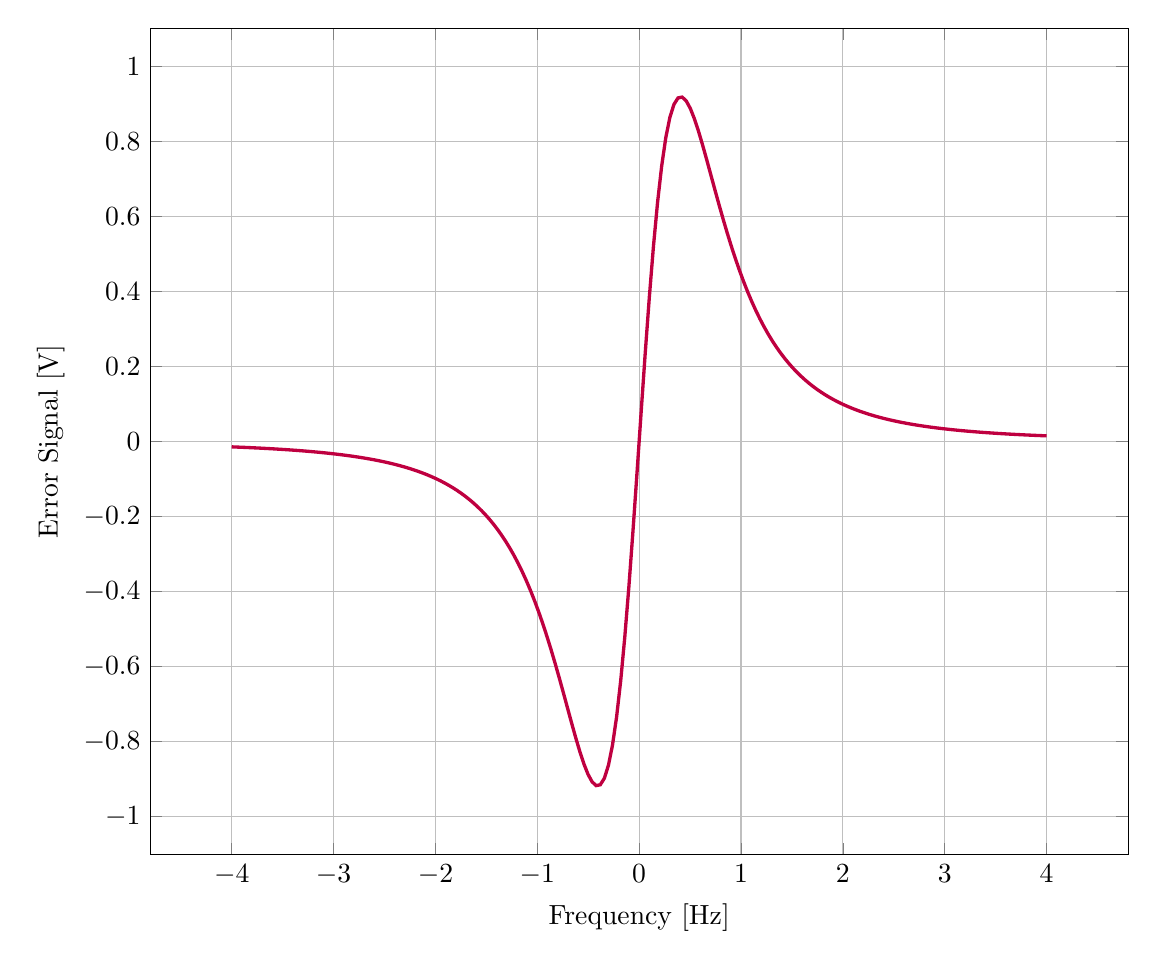
\begin{tikzpicture}
\begin{axis}[
    samples=200,
    grid=both,
    xlabel={Frequency $\left[\mathrm{Hz}\right]$},
    ylabel={Error Signal $\left[\mathrm{V}\right]$}
    ]
%  \addplot[blue,domain=-4:4,very thick] {x*exp(-x*x)};
  \addplot[purple,domain=-4:4,very thick] {x/(x*x+0.5)/(x*x+0.5)};
\end{axis}
\end{tikzpicture}
\caption[PDH Error Signal]{This shows the \ac{pdh} error signal of a simple
  cavity.
  Our lock point must be between the positive and negative cavity poles
  (maximum  and minimum on the y-axis).
  }
\label{fig:pdh}
\end{figure}

\subsubsection{Cavity Assembly}

The reference cavity is a Fabry Perot made from an 8 inch monolithic fused silica
spacer with high reflectivity mirrors glued onto the ends. The reflectivity
of the mirrors yield a finesse of about 7600. Finesse is defined as the ratio
of the \ac{fsr} to the cavity linewidth (\ac{fwhm}). One can arrive the
relationships between FSR, Finesse, mirror reflectivity as follows,
\begin{align}
E_{\mathrm{cavity}} =& E_{\mathrm{incident}} \sqrt{1-r_1^2} \left( 1 + r_1 r_2
    e^{i \omega 2 L /c} + \left(1+r_1 r_2 e^{i \omega 2L/c} \right)^2 + \ldots \right)
    \\
=& E_{\mathrm{incident}} \sqrt{1-r_1^2} \left( \frac{1}{1 - r_1 r_2
    e^{i \omega 2L/c}} \right)
\end{align}
Now, we find the reflected field,
\begin{align}
E_{\mathrm{reflected}} =& E_{\mathrm{incident}} \left( 1-r_1^2 \right)
    \left( \frac{r_2 e^{i \omega 2L/c}}{1 - r_1 r_2 e^{i \omega 2L/c}} \right)
    - r_1 E_{\mathrm{incident}}
\end{align}

\subsubsection{Cavity Suspension}
\begin{figure}[htbp]
	\centering
		\includegraphics[width=15cm]{./figures/refcavsusdesign.pdf}
	\caption[Reference Cavity Suspension Design]{Design of the reference cavity suspension}
	\label{fig:refcav_sus}
\end{figure}


\subsection{Feedback}
The feedback electronics used for the \ac{fss} are from initial LIGO. The board
provides feedback signal for 2 different actuation paths. The low frequency path
is to the laser cavity length which is split again into two different actuation
paths (thermal control and a piezo electric transducer in the laser head). The
other path is to an \ac{eom} to actuate on the phase of the laser beam.

\subsection{Actuation}

There are three actuators. Low frequency actuation is by a thermal controller in
the laser head which actuates on the the cavity length through thermal expansion.
The mid frequency actuation is by \ac{pzt} which applies a force to change the
cavity length. The high frequency actuation is by phase modulation of the light
after it exits the laser head using an \ac{eom}.

%\todopar{Add a description of the Electro-Optic Modulator}

%\subsubsection{Laser Head Thermal}
%
%\subsubsection{Laser Head Piezo-Electric Transducer}
%\todopar{add description of peizo-electric effect}
%\todopar{describe the effects of the piezo in-loop}

\subsubsection{Electro Optic Modulator}

\section{Mode Cleaner}
%\todopar{add description of PMC, reference Willke,98}
The PMC is a ring cavity of three mirrors.
see  \cite{Willke:98}


\subsection{Sensing}

\subsection{Feedback}

\subsection{Actuation}
Actuation on cavity length is done with a piezo-electric transducer on one of
the mirrors. This transducer converts voltage to cavity length.



\Chapter{Linear Trap Experiment}
\label{ch:lintrapex}

\section{Experimental Layout}

\section{High-Q Payload Suspension}

\section{Procedures}

\subsection{Measure the optical losses up to the cavity}

\subsection{Calibration of carrier and subcarrier photodiodes}
We will calibrate the photodiodes while the cavity is not locked, knowing the incident beam power and the round trip losses.

\begin{itemize}
    \item Block carrier light in Mach-Zehnder path.
    \item Turn the reflection monitor beam half-wave plate to minimize subcarrier light on the photodiode.
    \item Block the reflection monitor beam to measure dark voltage at DCPD ($A$).
    \item Unblock the reflection monitor beam and measure voltage at DCPD ($B$).
    \item Unblock the carrier light and measure again ($C$)
    \item Block subcarrier light and measure the carrier power using power meter after last steering mirror on table 1 ($D$).
    \item Using the measured optical loss to the cavity ($L$) compute the mW/mV calibration:
    \begin{itemize}
        \item $\frac{D\cdot L}{C - B}$
    \end{itemize}
\end{itemize}

\section{Mode Matching}
We want to know how much power couples into the cavity from a
perfectly gaussian beam of the wrong size and location. We start with
the equations for the Hermite-Gaussian beam expansion as discussed in
\cite{Siegman86}.

\newcommand{\intinfxy}[1]{\int^{\infty}_{- \infty} \int^{\infty}_{- \infty} #1 \,dx \,dy}
\newcommand{\intinfrt}[1]{\int^{2 \pi}_{0} \int^{\infty}_{0} #1 r \,dr \,d\theta}


\begin{align}
    c_{nm} &= \intinfxy{
    E(x,y,z) u_n^*(x,z)u_m^*(y,z)}
\\  &= \intinfxy{
    E(x,y,z) u_0^*(x,z)u_0^*(y,z)}
\\  &= \intinfxy{
    u_0(x,z-z_0)u_0(y,z-z_0) u_0^*(x,z)u_0^*(y,z)}
\\  &= \intinfxy{ \left( \frac{2}{\pi w^2_0} \right) \left( \frac{q_0}{q(z)} \right)
    \left( \frac{q^*_0}{q^*(z)} \right) \exp \left[-ik \left( x^2 + y^2  \right)
    \left( \frac{1}{2q(z)} + \frac{1}{2q^*(z)} \right) \right]}
\end{align}

Since $q(z) = q_0 + z - z_0$, and $q_0$ is purely imaginary,


\begin{multline}
    c_{00} = \intinfxy{ \left( \frac{2}{\pi w^2_0} \right)
    \left( \frac{-q^2_0}{(q_0+z-z_0)(-q_0+z)} \right) \\
    \exp \left[
    \frac{-ik \left( x^2 + y^2  \right)}{2} \left( \frac{(q_0+z-z_0)-(-q_0+z)}{(q_0+z-z_0)(-q_0+z)} \right)
    \right]}
\end{multline}

A careful analysis of the exponent will reveal that the real part must be greater than $0$.
We can therefore solve the Gaussian integral, setting $s = \frac{-ik \left( x^2 + y^2
\right)}{2} \left( \frac{(q_0+z-z_0)-(-q_0+z)}{(q_0+z-z_0)(-q_0+z)} \right)$

\begin{multline}
    c_{00} = \intinfrt{ \left( \frac{2}{\pi w^2_0} \right)
    \left( \frac{-q^2_0}{(q_0+z-z_0)(-q_0+z)} \right) \\
    \exp \left[
    \frac{-ik \left( r^2  \right)}{2} \left( \frac{(q_0+z-z_0)-(-q_0+z)}{(q_0+z-z_0)(-q_0+z)} \right)
    \right]}
\end{multline}

\begin{align}
    c_{00} &= \intinfrt{ \left( \frac{2}{\pi w^2_0} \right)
    \left( \frac{-q^2_0}{(q_0+z-z_0)(-q_0+z)} \right)
    \exp \left[
    s
    \right]}
\\  &= \int^{\infty}_{0} \left( \frac{4}{w^2_0} \right)
    \left( \frac{-q^2_0}{(q_0+z-z_0)(-q_0+z)} \right)
    \exp \left[
    s
    \right] r \,dr
\\  &= \int^{0}_{-\infty} \left( \frac{4}{w^2_0} \right)
    \left( \frac{-q^2_0}{(q_0+z-z_0)-(-q_0+z)} \right)
    \exp \left[ s
    \right] \frac{1}{-ik} \,ds
\\  &= \left( \frac{4i}{kw^2_0} \right)
    \left( \frac{-q^2_0}{(q_0+z-z_0)-(-q_0+z)} \right)
    \int^0_{-\infty} e^s \,ds
\\  &= \left( \frac{4i}{kw^2_0} \right)
    \left( \frac{-q^2_0}{2q_0-z_0} \right)
\\  &= \left( \frac{4i \lambda}{2 \pi w^2_0} \right)
    \left( \frac{-q^2_0}{2q_0-z_0} \right)
\\  &= \left( \frac{4i \lambda}{2 \pi w^2_0} \right)
    \left( \frac{-q_0 q_b}{2i \pi \omega^2_0 / \lambda - z_0} \right)
\\  &= \left( \frac{4i}{2 \lambda} \right)
    \left( \frac{\pi w_b^2}{2i \pi \omega^2_0 / \lambda - z_0} \right)
\\  &= 
    \frac{w_b^2}{\omega^2_0 + i z_0 \lambda /2 \pi}
\\  &= \frac{(w_b/w_0)^2}{1 + i z_0 /2 z_R}
\end{align}

Power coupling into cavity is then,
\begin{align}
P_{\mathrm{in cavity}} &= P_{\mathrm{incident}} \frac{(w_b/w_0)^4}{1+(z_0/2z_R)^2}
\end{align}



\Chapter{Digital System}
\label{ch:digital}

\section{System Overview}

\begin{figure}[htbp]
	\centering
		\includegraphics[width=15cm]{./figures/FrontEndSystem.pdf}
	\caption{{Front End System Overview}}
	\label{fig:front_end}
\end{figure}


\section{LIGO Real-Time System}

\section{ADC/DAC}

\section{Timing}

The timing signal for the front end system is directly generated by a Stanford Research DS345 function generator. It produces a 65,536 Hz signal that clocks the ADC and DAC cards. Over a long period of time the time stamp in the front end can drift relative to the computers that are synced to network time. Some software, particularly Diagnostic Test Tools and probably others, gets confused when the current time in front end does not match network time. This requires a reboot of the front end system to reacquire the correct time.

We ordered a GPS receiver (Trimble Thunderbolt E) that will prevent these long term drifts. It produces a 1PPS (Pulse Per Second) signal and a 10 MHz signal. The 1PPS connects to the ADC card through the ADC adapter card which is located in the blue expansion chassis. The 10 MHz signal connects to the external timebase input of the DS345. So, the 65,536 clock is now "disciplined" to the GPS time and as such should not drift over long periods of time.

Additionally, the Thunderbolt has an ovenized crystal oscillator that should help with phase noise.

In order to get the GPS antenna signal we needed about 250' of low-loss 1/2" diameter foam core cable (should be easy to spot as it's quite thick). The cable runs out the optics lab, across the hallway overhead and into a cable tray to go down the hallway. The cable runs out of the cable tray by the machine shop, over the hallway, into the machine shop, up to the ceiling, and then along the top of a black drain pipe to the south-east corner of the building. The cable then goes through some grating on the wall and up the shaft to the ground level of the SE corner where the antenna is mounted. (see Fig.\ref{fig:gps_antenna})

\begin{figure}[htbp]
	\centering
		\includegraphics[width=15cm]{./figures/IMG_1308.jpg}
	\caption{{GPS Antenna Location}}
	\label{fig:gps_antenna}
\end{figure}

The 1PPS signal from the Trimble Thunderbolt GPS receiver is a fixed pulse width of 10 micro-seconds. Since the clock is running at 65,536 Hz, the 1PPS is missed by the ADC.

I have fixed this by extending the pulse to about 15 microseconds using a 555 timer chip in monostable mode. The input has to be an inverse pulse so I inverted the pulse in GPS control software. This option is available in the Timing Receiver Configuration window.

See attached NE555P spec sheet (p.9) for the schematic that I used. Only difference is R\_L is between output and ground instead of V\_CC.

I scavenged a 5V power supply from an old 10baseT ethernet hub. I took the ferrites and electrolytic capacitor that were on the supply input in the hub itself and added them to this board for noise suppression.

R\_A is a small potentiometer. If you need to adjust the pulse width, just open the case and turn the pot. Clockwise increases the width.

\begin{figure}[htbp]
	\centering
		\includegraphics[width=15cm]{./figures/timer555.png}
	\caption{{555 Timer Diagram}}
	\label{fig:timer_diag}
\end{figure}


\begin{figure}[htbp]
	\centering
		\includegraphics[width=15cm]{./figures/IMG_1345.jpg}
	\caption{{GPS Pulse Extender}}
	\label{fig:gps_pulse}
\end{figure}

The first thing to check in the GPS software is the status. It should say "over-determined clock". Other key items in the control software to pay attention to are basically the number of green lights (in this case 5) and the holdover time in the upper-right window labeled "Timing Receiver Status and Control". If things are working correctly the number of green satellites will typically be 4-5 with the antenna at it's current location. We should also not see any holdover time. When the receiver is not using any satellites it enters a "holdover" state where the oscillator is no longer disciplining. The GPS keeps track of how long it's been in holdover. Going into holdover could indicate a problem in the connection to the GPS antenna.


\section{Hardware Integration}

\section{Code Installation}

We have acquired a clone of the front end disk used at Livingston. The disk was backed up locally (sugar-dev3:/lab/frontend/sata-disk-backups/mnt2 as of 2013/02/18). The disk was adapted for use at Syracuse. The disk failed on 6 Feb 2013. This page documents the second build of the front end at syracuse...




\section{Using LLO clone disk}



\subsection{LLO tar deploy}

Using the tar file from LLO...

\subsubsection{Local Disk Install}

\subsubsection{Diskless Node Install}

\begin{itemize}
    \item Acquire machine with same architecture as front-end (presumably x86\_64).
    \item Login using gentoo minimal-CD or Live-DVD.
    \item Repartition first disk (/dev/sda) to one partition and create ext3 filesystem.
    \item Make mount point for sda1 and mount.
%
\begin{lstlisting}
mkdir /mnt/fe
mount /dev/sda1 /mnt/fe
\end{lstlisting}
%
    \item Make mount point for /lab and mount directory.

\begin{lstlisting}
mkdir /mnt/lab
mount -t nfs 10.20.1.15:/sugwg/projects/lab /mnt/lab
\end{lstlisting}

    \item copy tar file:

\begin{lstlisting}
rsync -a /mnt/lab/frontend/sata-disk-backups/mnt2/fe.tar.gz /mnt/fe/
\end{lstlisting}

    \item untar file:

\begin{lstlisting}
cd /mnt
tar -xvf fe/fe.tar.gz
\end{lstlisting}

    \item chroot into new filesystem and setup for use on network...
\end{itemize}


\subsection{Minimal tar deploy}

Create a tar file without the portage, front-end target, and cvs/svn directories...

\subsubsection{Creating tar file for Syracuse front-end machine}

This is the procedure used to create an archive of a front-end system modified for use at Syracuse. Here, I am using 10.20.1.44 (s1boot0) as the machine to boot from (the tftp server) and 10.20.1.45 (s1labfe1) is the diskless front-end machine. This can easily be modified for installation directly onto the hard drive.

\begin{enumerate}
    \item Copy the fe tar file to \$\{FE\_LOCATION\} and untar.
\begin{lstlisting}
cd ${FE_LOCATION}
cp /lab/frontend/sata-disk-backups/mnt2/fe.tar.gz .
tar -xvpf fe.tar.gz
\end{lstlisting}
    \item \$\{FE\_LOCATION\}/fe is now the root directory for the front-end system
\begin{lstlisting}
export FE_ROOT=${FE_LOCATION}/fe
\end{lstlisting}
    \item At LLO the controls user has UID:GID = 1001:1001. Change this to 512:512 for Syracuse. (You must execute this as root)
\begin{lstlisting}
find ${FE_LOCATION} -xdev -user 1001 -print0 | xargs -0 chown 512:512
\end{lstlisting}
    \item Change the lines for controls in the files \$\{FE\_ROOT\}/etc/passwd and \$\{FE\_LOCATION\}/fe/etc/group
    \item Edit \$\{FE\_ROOT\}/etc/ntp.conf: Change "server" and "restrict" lines and comment out "broadcast" line
\begin{lstlisting}
server 10.20.1.25
restrict 10.20.1.0 mask 255.255.255.0 nomodify nopeer notrap
\end{lstlisting}
    \item Comment out entries in \$\{FE\_ROOT\}/etc/conf.d/net and add this line:
\begin{lstlisting}
config_eth4=( "10.20.1.45 netmask 255.255.0.0 broadcast 10.20.255.255" )
\end{lstlisting}
    \item Change ip address found in 3 files in \$\{FE\_ROOT\}/etc/xinetd.d/ from 10.144.0.0/24 to 10.20.1.0/24
    \item Comment out 3 lines in \$\{FE\_ROOT\}/etc/resolve.conf
    \item remove \$\{FE\_ROOT\}/opt/rtcds
\begin{lstlisting}
rm -rf ${FE_ROOT}/opt/rtcds
\end{lstlisting}
    \item Comment out all lines in fstab except for "shm" and add lines for root and lab.
\begin{lstlisting}
echo -e "10.20.1.44:/tftpboot/s1labfe1      /               nfs     sync,hard,intr,rw,nolock,rsize=8192,wsize=8192    0 0" >> ${FE_ROOT}/etc/fstab
echo -e "10.20.1.15:/sugwg/projects/lab     /lab            nfs     sync,hard,intr,rw,nolock,rsize=8192,wsize=8192    0 0\n" >> ${FE_ROOT}/etc/fstab
\end{lstlisting}
    \item Change EPICS\_CA\_ADDR\_LIST in \$\{FE\_ROOT\}/opt/cdscfg directory
\begin{lstlisting}
find /ligo/feback/fe/opt/cdscfg/ -type f -print0 | xargs -0 sed --in-place=.old s/10.144.0/10.20.255/g
\end{lstlisting}
    \item Comment out "source /opt/cdscfg/rtsetup.sh" from \$\{FE\_ROOT\}/home/controls/.bashrc and add the following lines in it's place:
\begin{lstlisting}
export IFO=X2
export ifo=x2
export SITE=TST
export site=tst
export RCG_LIB_PATH=/lab/frontend/controls/git/cds_user_apps/cds/b1/models
export RTCDSROOT=/opt/rtcds/${site}/${ifo}
export NDSSERVER=10.20.1.45:8088
export EPICS_CA_ADDR_LIST="10.20.255.255"
export EPICS_CA_AUTO_ADDR_LIST="NO"
export LD_LIBRARY_PATH=${LD_LIBRARY_PATH}:/lib:/usr/lib:/usr/local/lib:/opt/rtapps/fftw-3.2.2/lib
source /opt/rtapps/epics/etc/epics-user-env.sh
source /opt/rtapps/ldas-tools-1.18.2/etc/ldas-tools-user-env.sh
source /opt/rtapps/libframe-8.11/linux-x86_64/etc/libframe-user-env.sh
source /opt/rtapps/libmetaio-8.2/linux-x86_64/etc/libmetaio-user-env.sh
source /opt/rtapps/gds/etc/gds-user-env.sh
export PATH=${PATH}:/opt/rtapps/dv:/opt/rtcds/${site}/${ifo}/scripts
\end{lstlisting}
\end{enumerate}
\subsubsection{Creating a bootable disk for front-end}

This is how to build a disk that can be installed directly into a front-end machine.

*NOTE* The machine that you build this disk from must have the same type of disk controller as the front-end machine you intend to install this in.

\begin{enumerate}
    \item Locate a spare disk and install in a machine connected to the internal network that you have root access to.
    \item Mount /lab on this machine.
    \item Use fdisk or parted to partition the spare disk.
\begin{lstlisting}
Number  Start   End     Size    Type     File system     Flags
 1      512B    32.0MB  32.0MB  primary  ext2
 2      32.5MB  542MB   510MB   primary  linux-swap(v1)
 3      542MB   1000GB  1000GB  primary  ext4
\end{lstlisting}
    \item Mount /dev/sd* (blank spare disk) at /mnt/fe
\end{enumerate}


\Chapter{Noise Sources}
\label{ch:noises}
\section{Seismic}

\section{Thermal}

\section{Laser Frequency}

\section{Laser Intensity}

\section{Electronics}

\section{Residual Gas}

\section{Noise Budget}

\begin{figure}[htbp]
	\centering
		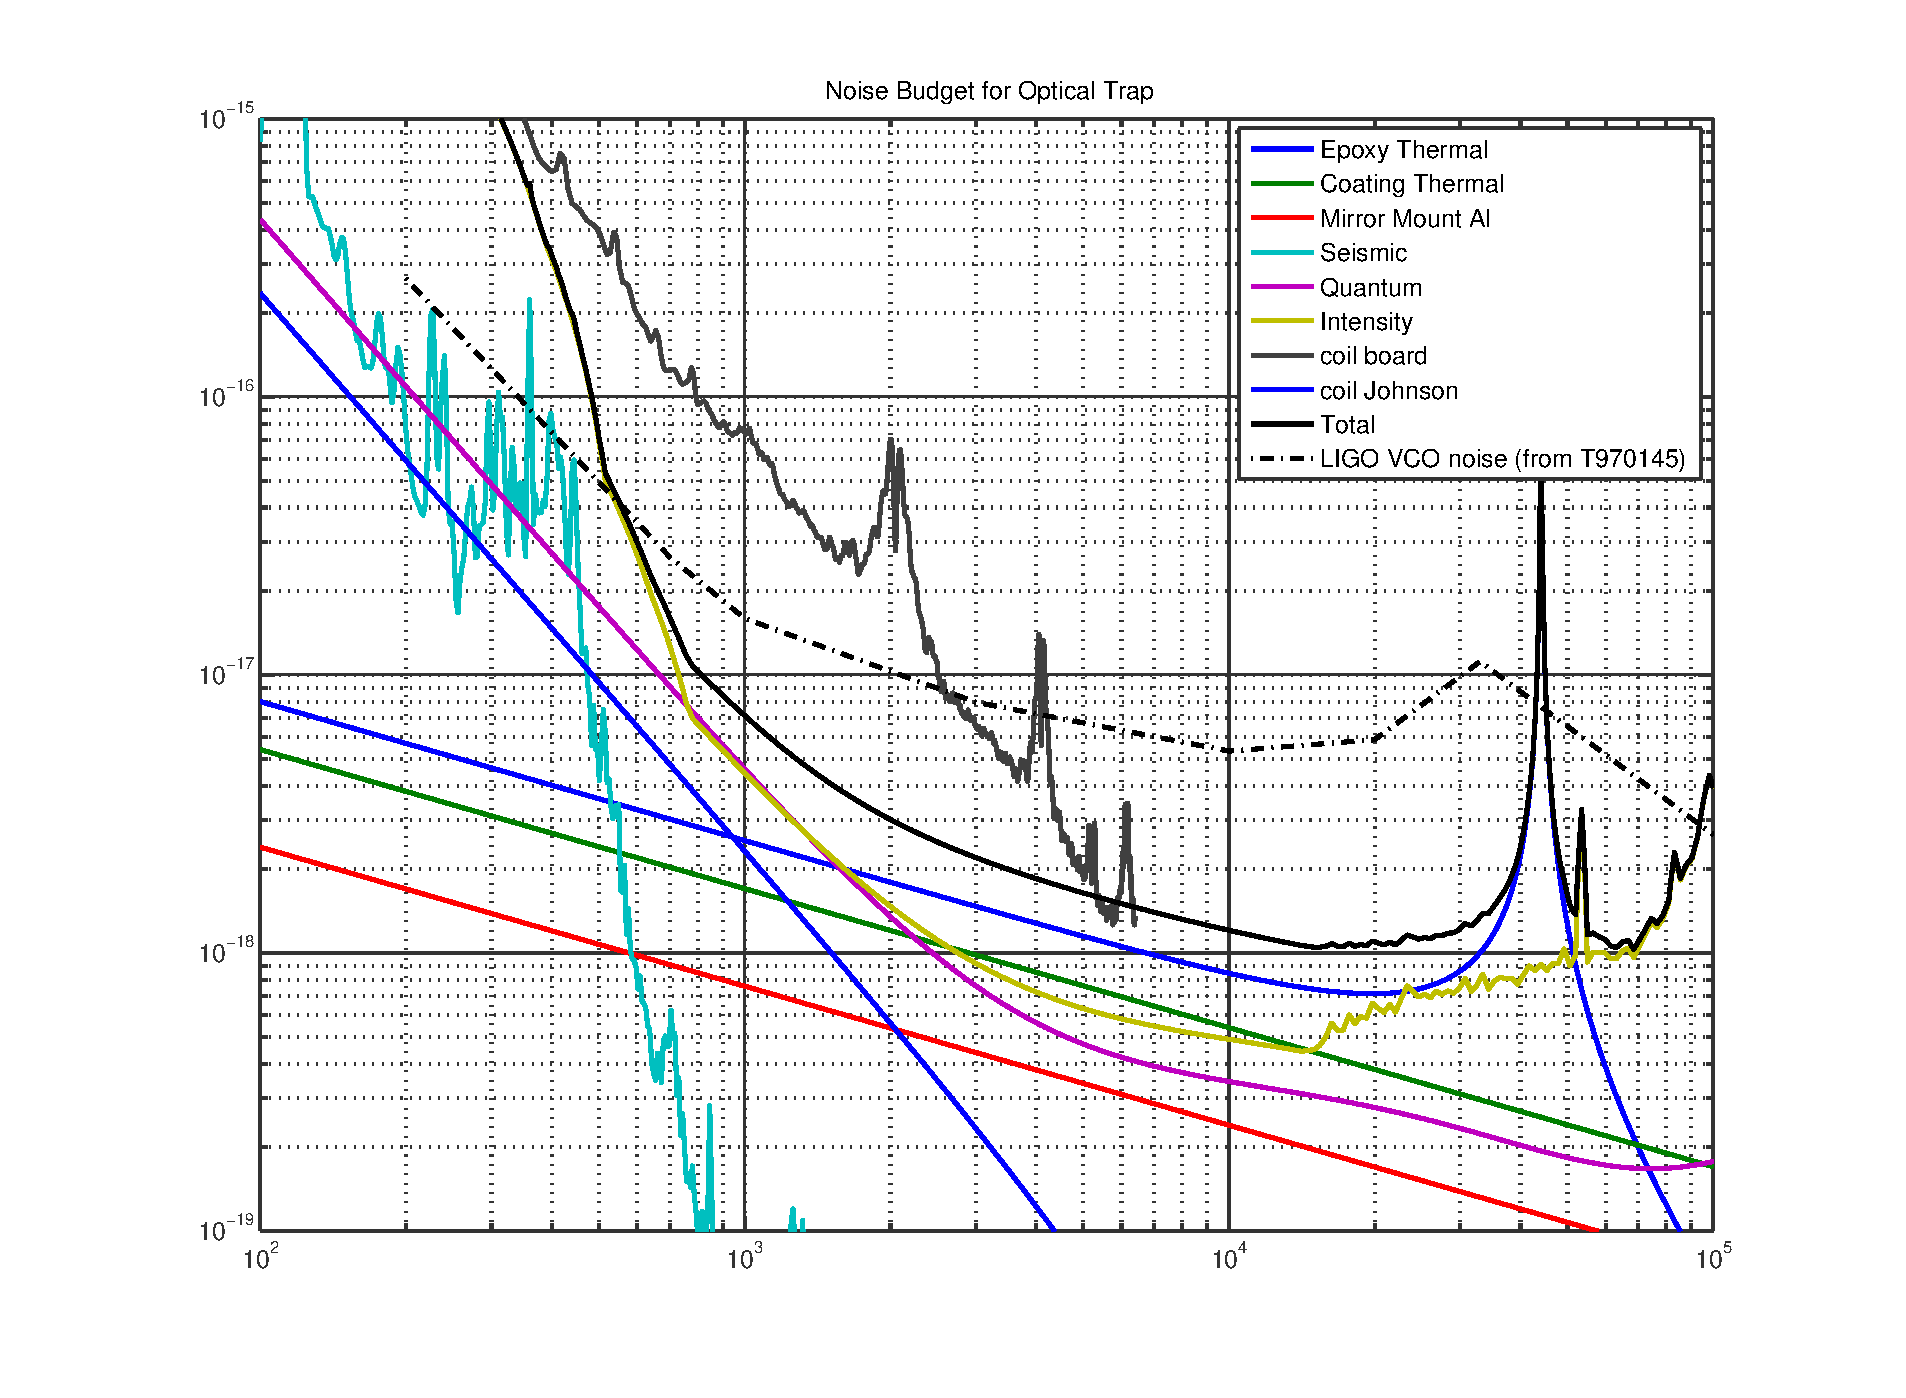
\includegraphics[width=15cm]{./figures/noise_budget.eps}
	\caption[Noise Budget]{Noise budget}
	\label{fig:noise_bud}
\end{figure}

\begin{figure}[htbp]
	\centering
		\includegraphics[width=15cm]{./figures/NoiseBudgetBoard.pdf}
	\caption[Noise Budget Board]{Noise budget with coil driver board noise}
	\label{fig:noise_bud_brd}
\end{figure}

\section{Vacuum Requirements for Optical Trap}

It is desired to have an understanding of limits of vacuum gas constituents for the in-vacuum experiment. From the LIGO DCC we have a few documents that describe the process that went into understanding the problem for 2 4km long Fabry-Perot cavities. I will apply these techniques to a 10-30cm cavity.\\


\subsection{LIGO Vacuum Requirements}

The amplitude spectral density of the optical path length is given by,

\begin{align*}
\Delta L ( f ) = 4 \pi \left( \frac{2 L_0 p}{k T w_0 v_0} \right)^{1/2} a e^{- \pi f w_0 / v_0 }
\end{align*} \\


From *** the value for $4 \pi a \left( \frac{2}{k T w_0 L_0 v_0} \right)^{1/2} $ is $ 4.8 x 10^{-21} \left( \frac{R_x}{R_{H_2}} \right) $. Where $L_0 = 4000 \mathrm{m} $ and $ w_0 = 0.06 \mathrm{m} $. \\

For our purposes (single arm cavity) we will lose a factor of $ \sqrt{2} $. \\

We end up with a formula for amplitude spectral density in a one-arm cavity that is:

\begin{align*}
\Delta L ( f ) = 4 \pi \left( 5.3 \mathrm{x} 10^{-20} \right) \left(  \frac{R_x}{R_{H_2}} \right) \sqrt{\frac{ L_0 p}{ w_0 } } e^{- \pi f w_0 / v_0 }
\end{align*} \\

\subsection{Optical Trap}

Now, we insert parameters for the cavity. For the first look, I use the parameters defined in the project description: 0.3m cavity length, 0.2m radius of curvature for each mirror.
\todo{something},

If we operate at a pressure of 1e-6 Torr, no constituent gas can be greater than this. The following plot is of constituent gases at this pressure.

\begin{figure}[htbp]
	\centering
		\includegraphics[width=15cm]{./figures/trapgasnoise_1.png}
	\caption[Gas Noise Comparison]{Gas Noise for 1e-6 Torr}
	\label{fig:gas_noise1}
\end{figure}

If we have a residual gas analyzer that detects a minimum partial pressure of 5e-11 Torr:

\begin{figure}[htbp]
	\centering
		\includegraphics[width=15cm]{./figures/trapgasnoise_2.png}
	\caption[Gas Noise Comparison]{Gas Noise for 5e-11 Torr}
	\label{fig:gas_noise2}
\end{figure}

\section{Epoxy Thermal Noise}

Brownian thermal noise estimates for epoxy joints are gotten from basic application of the fluctuation-dissipation theorem. The form that we start with is,
\begin{align*}
S_{x^2}(f) = \frac{4 k_B T}{\omega^2} \Re(Z^{-1}), 
\end{align*}
where $Z$ is the impedance, $F / v$. The force equation that we use is of the form,
\begin{align*}
F_{\mathrm{ext}} = m \ddot{x} + k x,
\text{where k is a complex number}, (1 + i \phi)
\end{align*}

\section{Derivation}

\begin{align*}
d_n = d(t-\tau_n)
\end{align*} \\

\begin{align*}
d_n = d \left( t - \frac{(2n -1)}{c} L_0 - d_1 - \sum_{l=2}^{n} 2 d_l \right)
\end{align*} \\



%\Chapter{Feedback Control}
%\label{ch:feedback}
%\input(feedback.tex}


\clearpage
\bibliographystyle{unsrt}
\bibliography{OT_paper,references}
\addcontentsline{toc}{chapter}{\numberline {Bibliography}}

\clearpage
\birthplacedate{Blacksburg, Virginia \>\>August 30, 1973}
\collegewherewhen{
\>Virginia Tech \>\>B.S. Physics, 2001}

\newpage
\null%\vskip1in%
\begin{center}
{\Large\bf Vita}
\end{center}

\begin{startvita}
\end{startvita}

\renewenvironment{thebibliography}[1]%
  {\begin{list}{\labelenumi\hss}%
     {\usecounter{enumi}\setlength{\labelwidth}{3em}%
      \setlength{\leftmargin}{5em}}}%
  {\end{list}}
\renewcommand{\bibitem}[1]{\item\label{#1}\relax}%
\renewcommand{\theenumi}{\arabic{enumi}}%
\begin{publications}
\putbib[papers]
\end{publications}

\begin{honorarysocieties}
\end{honorarysocieties}


\end{document}
